\documentclass[12pt,a4paper]{article}

\usepackage[utf8]{inputenc}
\usepackage[T1]{fontenc}
\usepackage[brazil]{babel}
\usepackage{geometry}
\usepackage{graphicx}
\usepackage{booktabs}
\usepackage{longtable}
\usepackage{array}
\usepackage{float}
\usepackage{hyperref}
\usepackage{xcolor}

\geometry{margin=2.5cm}
\setlength{\parindent}{0pt}
\setlength{\parskip}{0.65em}
\renewcommand{\arraystretch}{1.15}

\hypersetup{
    colorlinks=true,
    linkcolor=blue,
    urlcolor=blue,
    citecolor=blue
}

\title{Racional técnico para seleção de consórcios microbianos orientados à degradação de compostos alifáticos e poliaromáticos}
\author{BioRemPP -- Modelagem de consórcios}
\date{\today}

\begin{document}

\maketitle

\begin{abstract}
Este documento consolida o racional técnico usado para selecionar dois consórcios microbianos candidatos: um orientado a compostos alifáticos e outro a compostos poliaromáticos. A seleção combinou cobertura anotacional de compostos, agrupamento por guildas funcionais, completude de KOs, evidência de inventário gênico, diversidade de atividades enzimáticas, métricas de mitigação de risco e resultados experimentais por DCPIP. O documento também propõe um consórcio controle negativo composto por \textbf{BD2} e \textbf{BD161}, aplicável aos ensaios alifáticos e poliaromáticos, por combinar menor suporte genômico relativo com menor desempenho experimental.
\end{abstract}

\section{Objetivo e lógica geral da seleção}

O objetivo da análise foi transformar um conjunto amplo de isolados com evidências genômicas e experimentais em dois consórcios candidatos, cada um com função definida:

\begin{itemize}
    \item \textbf{Consórcio alifático}: \textbf{BD163}, \textbf{BD127}, \textbf{E7} e \textbf{BD117}.
    \item \textbf{Consórcio poliaromático}: \textbf{BD61}, \textbf{BD120}, \textbf{BD158} e \textbf{BD117}.
    \item \textbf{Consórcio controle negativo}: \textbf{BD2} e \textbf{BD161}, proposto para ambos os eixos experimentais.
\end{itemize}

A estratégia adotada não buscou apenas selecionar isolados com maior número absoluto de genes ou maior resposta experimental isolada. O critério central foi a convergência entre três camadas de evidência: cobertura de compostos, complementaridade funcional e suporte experimental por DCPIP.

\section{Filtro por resistência a metais como critério de robustez}

Antes de selecionar os consórcios orientados a hidrocarbonetos, foi utilizado um universo elegível derivado da visualização de UC 8.1 para a classe Metal. Esse passo foi interpretado como um critério de robustez associado à \textbf{resistência a metais}, e não como uma seleção por potencial de degradação de metais. A lógica biológica é que isolados capazes de compor uma solução funcional em um eixo de estresse por metais podem ser candidatos mais robustos para ambientes contaminados complexos, como matrizes petrolíferas que combinam hidrocarbonetos e pressões inorgânicas.

A Figura~\ref{fig:metal} resume esse universo elegível. Ela foi usada como fonte de autoridade para a composição dos grupos funcionais de Metal.

\begin{figure}[H]
    \centering
    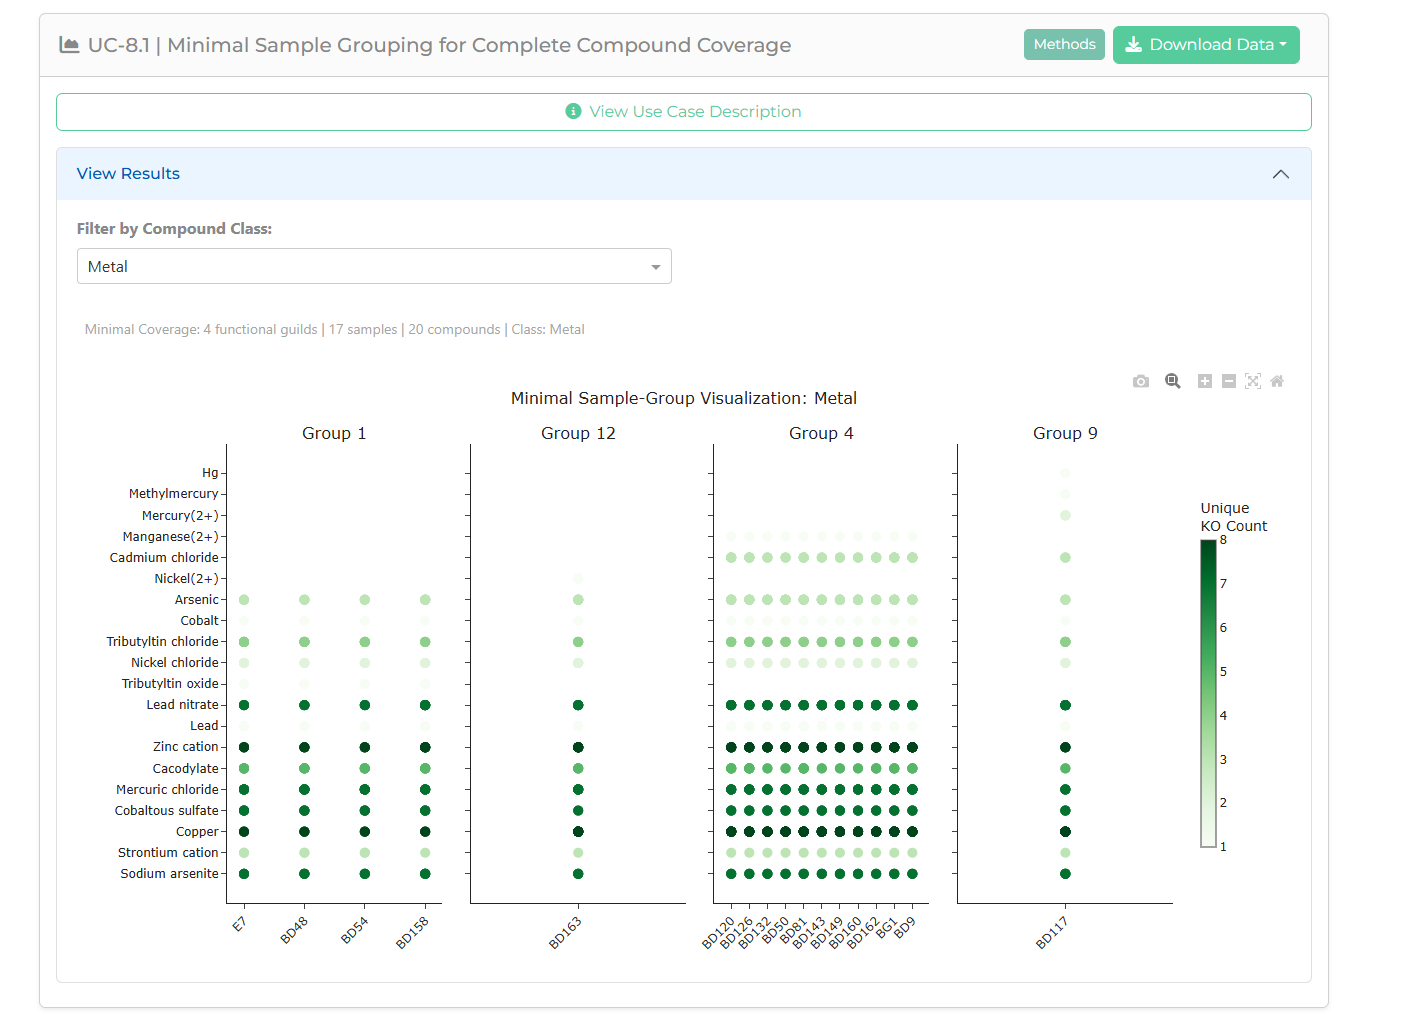
\includegraphics[width=0.95\textwidth]{UC_8.1/UC8.1_METAL.png}
    \caption{Agrupamento mínimo de amostras para cobertura de compostos da classe Metal. Nesta análise, a figura foi usada como referência para o universo de isolados elegíveis sob o critério de resistência a metais.}
    \label{fig:metal}
\end{figure}

Esse filtro produziu um conjunto de isolados candidatos que foram posteriormente reavaliados quanto à cobertura de compostos alifáticos e poliaromáticos. Assim, a resistência a metais funcionou como um critério anterior de elegibilidade e consistência ambiental, enquanto a escolha final de cada consórcio foi guiada pela cobertura de hidrocarbonetos e pelo suporte experimental.

\section{Metodologia de priorização}

Para cada classe-alvo, os isolados foram comparados por perfis de cobertura de compostos. Isolados com perfis equivalentes foram tratados como membros de uma mesma guilda funcional. A seleção buscou representar as guildas necessárias para maximizar a cobertura total da classe química com o menor número de membros.

Quando uma guilda tinha mais de um candidato funcionalmente equivalente, o DCPIP foi usado como critério experimental de desempate. Para compostos alifáticos, a métrica mais relevante foi a média de petróleo leve (\texttt{PL\_mean}). Para compostos poliaromáticos, a métrica mais relevante foi a média de petróleo pesado (\texttt{PP\_mean}). A média geral (\texttt{overall\_mean}) foi usada como suporte adicional.

As principais métricas usadas foram:

\begin{itemize}
    \item número de compostos cobertos pela combinação de isolados;
    \item número de novos compostos adicionados por cada representante;
    \item completude de KOs por classe;
    \item desempenho DCPIP em petróleo leve e pesado;
    \item inventário gênico e interseções de KOs entre os membros;
    \item amplitude e profundidade de mitigação de risco.
\end{itemize}

\section{Consórcio orientado a compostos alifáticos}

O consórcio alifático selecionado foi composto por \textbf{BD163}, \textbf{BD127}, \textbf{E7} e \textbf{BD117}. A combinação cobre \textbf{56 de 59 compostos alifáticos}, correspondendo a \textbf{94,92\%} de cobertura anotacional.

\begin{figure}[H]
    \centering
    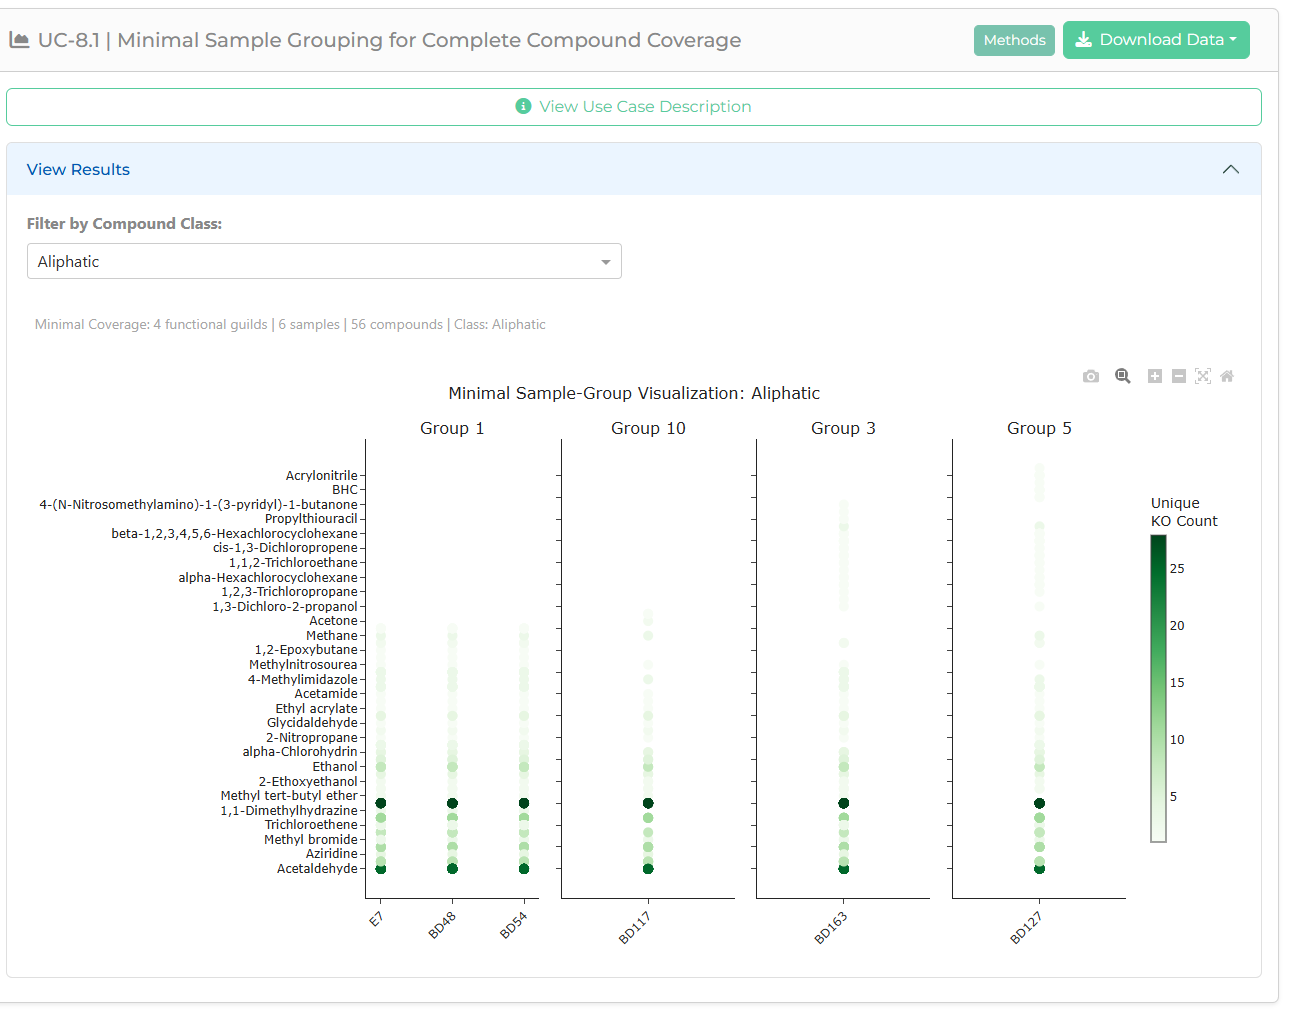
\includegraphics[width=0.95\textwidth]{UC_8.1/UC8.1_ALIPHATIC.png}
    \caption{Agrupamento mínimo de amostras para cobertura de compostos alifáticos dentro do universo elegível.}
    \label{fig:aliphatic}
\end{figure}

\begin{longtable}{p{1.8cm}p{2.7cm}p{2.1cm}p{2.1cm}p{2.1cm}p{4.0cm}}
\caption{Contribuição dos isolados no consórcio alifático.}\\
\toprule
\textbf{Isolado} & \textbf{Táxon} & \textbf{Novos compostos} & \textbf{PL médio} & \textbf{Completude KO} & \textbf{Interpretação} \\
\midrule
\endfirsthead
\toprule
\textbf{Isolado} & \textbf{Táxon} & \textbf{Novos compostos} & \textbf{PL médio} & \textbf{Completude KO} & \textbf{Interpretação} \\
\midrule
\endhead
BD163 & \textit{Bacillus megaterium} & 43 & 64,05 & 41,83\% & Núcleo de maior amplitude para compostos alifáticos. \\
BD127 & \textit{Achromobacter} & 7 & 59,21 & 36,60\% & Complementa a cobertura inicial e amplia o repertório funcional. \\
E7 & \textit{Acinetobacter} & 4 & 82,91 & 39,22\% & Representante experimentalmente mais forte da guilda com múltiplos candidatos. \\
BD117 & \textit{Micococcus luteus} & 2 & 79,18 & 25,49\% & Membro complementar, com alta sustentação experimental por DCPIP. \\
\bottomrule
\end{longtable}

O caso mais importante de desempate ocorreu na guilda em que \textbf{E7}, \textbf{BD48} e \textbf{BD54} tinham papel anotacional equivalente. Nessa situação, a escolha de \textbf{E7} foi sustentada pelo maior \texttt{PL\_mean} entre os candidatos, com valor de \textbf{82,91}. \textbf{BD54} apresentou desempenho muito próximo em petróleo leve (\textbf{82,23}) e maior desempenho em petróleo pesado (\textbf{69,69}), mas o objetivo principal deste consórcio foi maximizar a coerência com a classe alifática, para a qual o petróleo leve foi usado como eixo experimental prioritário.

\section{Consórcio orientado a compostos poliaromáticos}

O consórcio poliaromático selecionado foi composto por \textbf{BD61}, \textbf{BD120}, \textbf{BD158} e \textbf{BD117}. A combinação cobre \textbf{43 de 44 compostos poliaromáticos}, correspondendo a \textbf{97,73\%} de cobertura anotacional.

\begin{figure}[H]
    \centering
    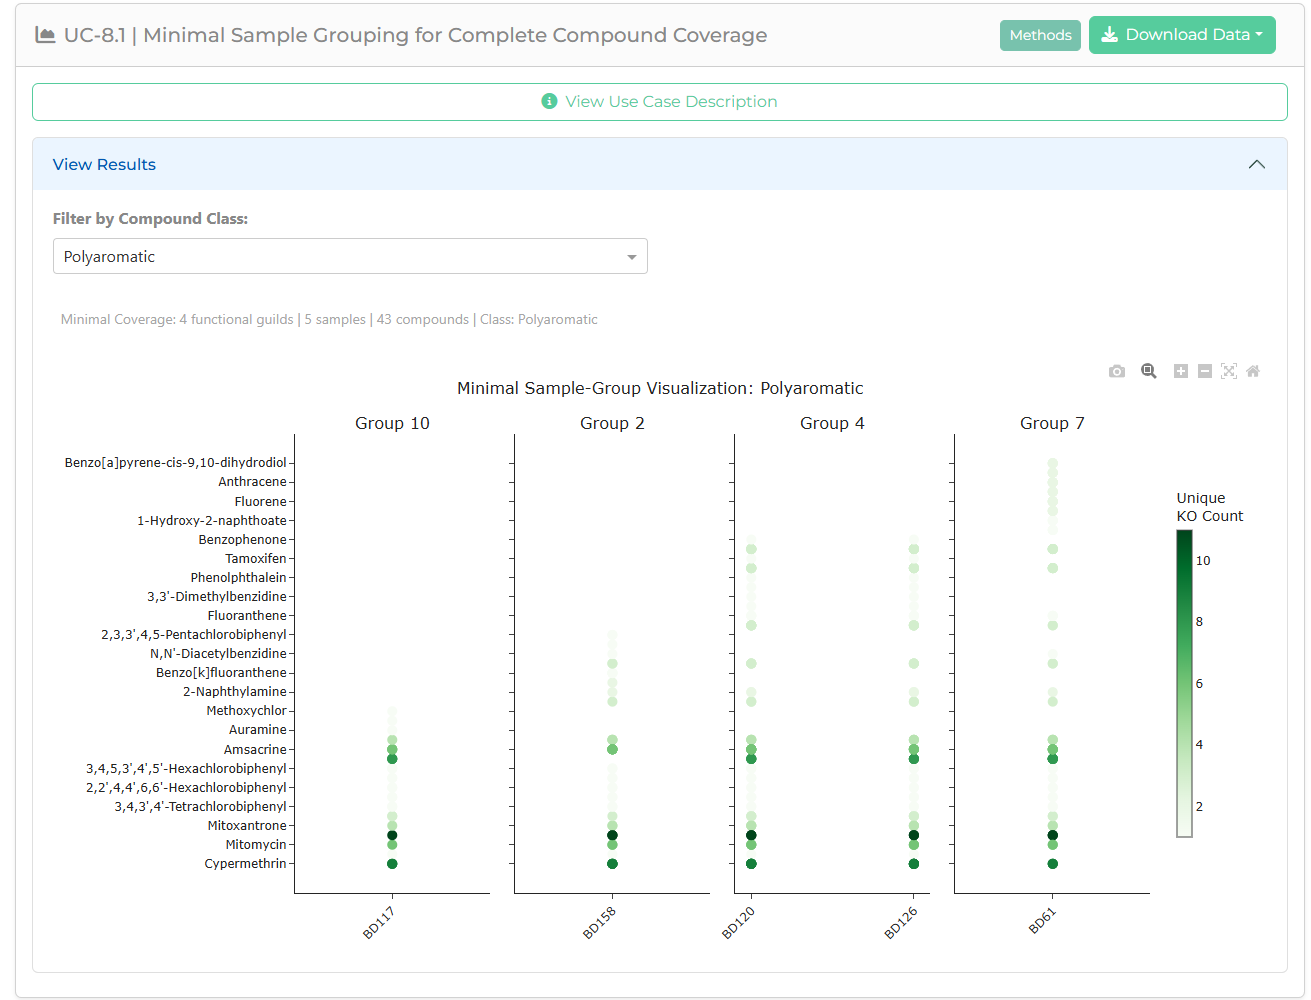
\includegraphics[width=0.95\textwidth]{UC_8.1/UC8.1_POLYAROMATIC.png}
    \caption{Agrupamento mínimo de amostras para cobertura de compostos poliaromáticos dentro do universo elegível.}
    \label{fig:polyaromatic}
\end{figure}

\begin{longtable}{p{1.8cm}p{2.7cm}p{2.1cm}p{2.1cm}p{2.1cm}p{4.0cm}}
\caption{Contribuição dos isolados no consórcio poliaromático.}\\
\toprule
\textbf{Isolado} & \textbf{Táxon} & \textbf{Novos compostos} & \textbf{PP médio} & \textbf{Completude KO} & \textbf{Interpretação} \\
\midrule
\endfirsthead
\toprule
\textbf{Isolado} & \textbf{Táxon} & \textbf{Novos compostos} & \textbf{PP médio} & \textbf{Completude KO} & \textbf{Interpretação} \\
\midrule
\endhead
BD61 & \textit{Ochrobactrum} & 29 & 59,63 & 40,96\% & Núcleo de maior ganho inicial para compostos poliaromáticos. \\
BD120 & \textit{Bacillus subtilis} & 7 & 81,81 & 48,19\% & Representante escolhido por forte desempenho experimental em petróleo pesado. \\
BD158 & \textit{Salinicola} & 4 & 58,54 & 37,35\% & Complementa cobertura e amplia repertório funcional. \\
BD117 & \textit{Micococcus luteus} & 3 & 76,65 & 22,89\% & Perfil complementar com alto desempenho experimental. \\
\bottomrule
\end{longtable}

O principal desempate ocorreu na guilda em que \textbf{BD120} e \textbf{BD126} exerciam o mesmo papel funcional. A escolha de \textbf{BD120} foi direta: ele apresentou \texttt{PP\_mean} de \textbf{81,81} e \texttt{overall\_mean} de \textbf{82,89}, enquanto \textbf{BD126} apresentou \texttt{PP\_mean} de \textbf{39,05} e \texttt{overall\_mean} de \textbf{49,66}. Como os dois eram funcionalmente equivalentes na guilda, o desempenho experimental tornou \textbf{BD120} o representante mais plausível para o eixo poliaromático.

\section{Evidências complementares de suporte}

As análises de suporte reforçam que os consórcios não foram selecionados apenas por presença ou ausência de anotações. O conjunto de evidências indica complementaridade funcional entre os membros.

\begin{longtable}{p{2.4cm}p{5.3cm}p{6.4cm}}
\caption{Síntese das evidências complementares usadas para sustentar a seleção.}\\
\toprule
\textbf{Evidência} & \textbf{Leitura técnica} & \textbf{Contribuição para a decisão} \\
\midrule
\endfirsthead
\toprule
\textbf{Evidência} & \textbf{Leitura técnica} & \textbf{Contribuição para a decisão} \\
\midrule
\endhead
UC 8.2 & Completude por classe química. & Mostra que os isolados mantêm suporte distribuído para as classes-alvo e para classes associadas ao contexto ambiental. \\
UC 8.3 & Completude KO por composto. & Evidencia heterogeneidade entre compostos, sustentando a necessidade de consórcios em vez de isolados únicos. \\
UC 8.7 & Interseção de KOs entre membros. & Mostra sobreposição parcial, combinando redundância funcional com especialização. \\
UC 4.8 & Inventário gênico por amostra. & Confirma repertórios amplos em BD127, BD163, E7, BD61, BD120 e BD158, com BD117 como membro mais compacto e complementar. \\
UC 4.10 & Diversidade de atividades enzimáticas. & Apoia a presença de atividades compatíveis com transformação de compostos, incluindo desidrogenases, dioxigenases e oxidoredutases. \\
UC 7.6 e UC 7.7 & Mitigação de risco e profundidade por investimento genético. & Reforça que os membros selecionados carregam repertórios relevantes para compostos de risco e pressões ambientais. \\
\bottomrule
\end{longtable}

No consórcio alifático, os tamanhos de conjuntos observados na análise de interseção foram aproximadamente \textbf{BD127 = 233}, \textbf{BD163 = 223}, \textbf{E7 = 221} e \textbf{BD117 = 153}. No consórcio poliaromático, os valores foram aproximadamente \textbf{BD61 = 229}, \textbf{BD158 = 227}, \textbf{BD120 = 217} e \textbf{BD117 = 153}. Esses resultados indicam que os membros compartilham um núcleo funcional, mas preservam contribuições específicas.

\section{Papel transversal de BD117}

\textbf{BD117} aparece nos dois consórcios porque ocupa uma posição complementar. Embora não seja o isolado de maior inventário gênico, ele adiciona compostos residuais não cobertos pelos membros principais e apresenta alto desempenho experimental em ambos os eixos.

\begin{table}[H]
\centering
\caption{Desempenho DCPIP de BD117.}
\begin{tabular}{lccc}
\toprule
\textbf{Isolado} & \textbf{PL médio} & \textbf{PP médio} & \textbf{Média geral} \\
\midrule
BD117 & 79,18 & 76,65 & 77,92 \\
\bottomrule
\end{tabular}
\end{table}

Essa combinação faz de \textbf{BD117} um isolado de ponte entre a lógica anotacional e a evidência experimental. Ele atua como componente de nicho, acrescentando cobertura funcional e aumentando a plausibilidade experimental dos consórcios.

\section{Consórcio controle negativo}

Para testar experimentalmente se menor repertório genômico nas classes de interesse acompanha menor degradação, foi proposto um consórcio controle negativo com dois isolados: \textbf{BD2} e \textbf{BD161}. Esse consórcio pode ser usado tanto nos ensaios alifáticos quanto nos ensaios poliaromáticos.

\begin{table}[H]
\centering
\small
\caption{Composição proposta para o consórcio controle negativo.}
\begin{tabular}{llccccc}
\toprule
\textbf{Isolado} & \textbf{Táxon} & \textbf{Genes alif.} & \textbf{Genes arom.} & \textbf{PL médio} & \textbf{PP médio} & \textbf{Média geral} \\
\midrule
BD2 & \textit{Staphylococcus} & 35 & 23 & 28,31 & 11,99 & 22,87 \\
BD161 & \textit{Rossellomorea} & 50 & 33 & 32,67 & 47,57 & 40,12 \\
\bottomrule
\end{tabular}
\normalsize
\end{table}

\textbf{BD2} é o membro mais forte como controle negativo, pois combina baixa contagem de genes para as classes alifática e aromática com o menor desempenho DCPIP observado entre os candidatos prioritários. \textbf{BD161} complementa o controle por apresentar baixo \texttt{PL\_mean} e baixa/intermediária contagem gênica, compondo um controle negativo de dois membros mais estável do que um isolado único.

É importante destacar que a análise global de correlação entre contagem gênica e DCPIP foi fraca. Para Aliphatic versus \texttt{PL\_mean}, o coeficiente de Spearman foi aproximadamente \textbf{-0,057}; para Aromatic versus \texttt{PP\_mean}, foi aproximadamente \textbf{-0,122}. Portanto, a hipótese não deve ser formulada como uma relação linear simples. O teste experimental mais defensável é comparar os consórcios selecionados contra um controle negativo que reúna, ao mesmo tempo, menor repertório anotacional e menor resposta DCPIP.

\section{Síntese final}

Os dois consórcios selecionados representam soluções complementares para dois eixos de degradação em matriz petrolífera:

\begin{itemize}
    \item \textbf{BD163 + BD127 + E7 + BD117}: consórcio orientado a compostos alifáticos, com alta cobertura anotacional, suporte experimental em petróleo leve e complementaridade entre guildas.
    \item \textbf{BD61 + BD120 + BD158 + BD117}: consórcio orientado a compostos poliaromáticos, com cobertura quase completa, forte suporte experimental em petróleo pesado e contribuição complementar entre membros.
    \item \textbf{BD2 + BD161}: consórcio controle negativo proposto para testar se perfis com menor suporte genômico e menor DCPIP resultam em menor degradação experimental.
\end{itemize}

A principal força do racional é a convergência entre evidências independentes. A cobertura de compostos define a arquitetura mínima dos consórcios; o DCPIP orienta a escolha entre candidatos funcionalmente equivalentes; e os casos de uso complementares sustentam que os isolados selecionados carregam repertórios gênicos, enzimáticos e de mitigação de risco coerentes com o uso pretendido.

\end{document}
